\documentclass[a4paper,10pt,twocolumn]{article}
\usepackage{fullpage}
\usepackage{hyperref}
\usepackage{epsfig}
\usepackage{graphicx}
\usepackage{caption}
\usepackage{subcaption}

\usepackage{stfloats}

\begin{document}

\title{{\bf EnRoute 2.0 - The HVAC Test-Bed} \\ \normalsize\url{''https://github.com/ESE519/EnRoute-2.0/wiki/_pages''}}
\date{December 15, 2012}
\author{Dan Wheeler \\dwheeler@seas.upenn.edu
        \and Larry Vadakedathu \\vlarry@seas.upenn.edu
	\and Neel D Shah \\neeldshah88@gmail.com}
\maketitle

\begin{figure}[ht]
\centering
\epsfig{file=enroute2.eps,width=\linewidth,clip=}
\caption{EnRoute2.0 Complete Assembly}
\label{enroute2}
\end{figure}

\vspace{-5 mm}

\begin{center}
{\bf Introduction}
\end{center}

EnRoute 2.0, as seen in \ref{enroute2}, is an expansion project based on previous work--EnRoute:  The Energy Router Test-Bed--which was aimed at creating a building simulation test-bed for the testing of control algorithms with the goal of improvements in energy scheduling and peak power reduction.  EnRoute 2.0 hopes to expand on the original project through two major components:  creating a more realistic test-bed more closely related to real world HVAC systems, and allowing anyone to run simulations on the test-bed remotely.  The first task is achieved largely through the introduction of ductwork with Variable Air Volume (VAV) control to each room handled through small servo valves and an Air Handling Unit (AHU) distributing air, reclaiming air, and recycling air.  Remote operation is achieved with IP communication using a static IP address supplied specifically for the master mBed controller of the system.

For large scale buildings, electricity costs vary with time based on total demand of the aggregate of consumers.  In such a scenario, energy can cost up to 200 times as much during peak operating hours as it does during normal operating conditions, or during the night when energy is at its cheapest due to low overall demand.  Additionally, peaks in power consumption of an individual facility can result in costly fines.  Therefore, if you can schedule your energy use efficiently to (1) avoid peaks in individual power, and (2) minimize the total power consumption during peak operating hours you could significantly reduce the total cost of electricity incurred.

Unfortunately, current systems are not designed to provide this type of operation.  Firstly, control units have no knowledge of how electricity costs are changing with time, and secondly, units operate almost entirely independent of each other.  We can view the second scenario in the case of cooling two rooms.  Initially one room is cooling while the other room is within its bounds for temperature control, therefore the system is only using approximately half its total power.  If the second room reaches its high threshold point it will switch on and both rooms will begin to cool.  If systems had an overall notion of what other nodes were doing it would be able to schedule the energy use so that all rooms stay within specified bounds, but also ensure that the system is not operating at maximum power if it does not need to be.

\begin{center}
{\bf Project Goals}
\end{center}

The first EnRoute project utilized four (4) mutually exclusive zones which were heated using incandescent lightbulbs with operation points at 0\%, 25\%, 50\%, 75\%, and 100\% of total power.  Cooling was not successfully implemented here, rather it was simulated by heating up the rooms and 'cooling' them by exhausting the warm air to the outside.  While algorithms were effectively developed on this system it lacked reality when compared to real-world buildings which most often achieve heating and cooling through HVAC units which deliver temperature controlled air from the unit itself to multiple rooms.  To improve the realistic aspects of this project we set out to design a system which mimicked an actual HVAC system as best we could as well as to provide methods for cooling.

\begin{figure}[t]
\centering
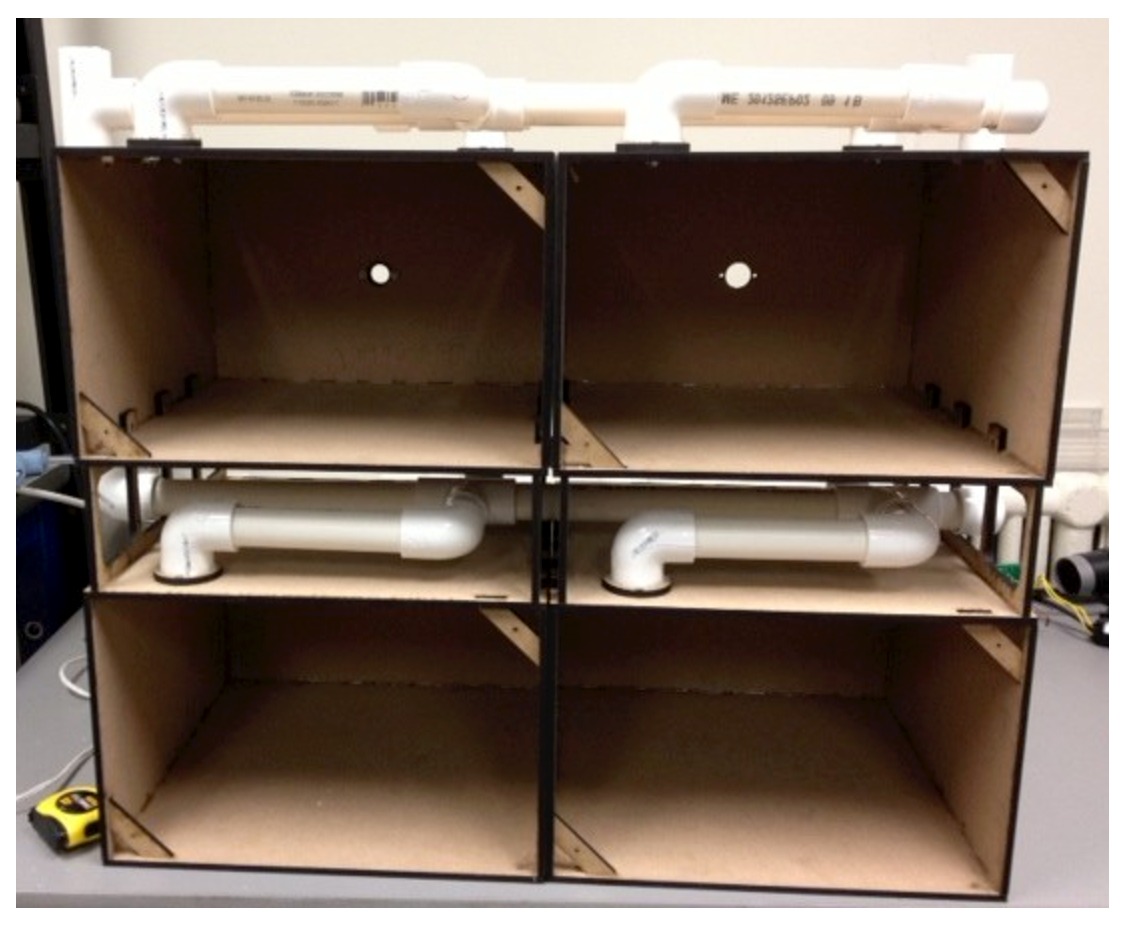
\epsfig{file=front.eps,width=0.8\linewidth,clip=}
\caption{View of All Zones}
\label{front}
\end{figure}

Firstly, an understanding of HVAC systems is critical to grasp what we wanted to achieve with this test-bed.  At the heart of every HVAC system is the Air Handler Unit (AHU) which has three main functions:  supply air to the ductwork using a blower, pull air from the rooms using a second blower, and allow for the ability to recycle air back into the HVAC.  Next most important are the cooling and heating coils, which are frequently (depending on the size of the system) located coaxially in the HVAC unit so that air is pulled over both coils in series.  A third important feature, which becomes critical for peak energy reduction, is the Variable Air Volume (VAV) control of the system which changes the amount of air pumped into the ductwork based on how much flow each room is requesting.  Our design seeks to meet all three of the goals with the implementation of an AHU, both heating and cooling elements, and VAV control.

The next goal of this project was aimed not only at creating a test-bed, but an open-source test-bed which could be used by anyone (assuming permission is given) to run their own simulations remotely (i.e. from anywhere in the world).  

\begin{center}
{\bf Hardware:  Structural Design and Implementation}
\end{center}

\emph{Zone Design:}
Building off of the general architecture of the original EnRoute model, we decided to proceed with the four room, two floor building model seen in \ref{front}.  We will refer to these floors as ‘zones’ in this project.  All four rooms were built with the same dimensions of 14.5" by 14.5" by 9.5" for better analysis of control algorithms.  These zones were completely laser cut out of quarter-inch medium density fiberboard (MDF) and held together by press fitting the edges.  The two zones are spaced four inches apart using a custom built bridge that aids the passage of necessary ductwork to and from each room.  In addition to this, we built completely detachable doors of 13.98" by 8.98" for the rooms which were also press fit to have minimal leakage from the rooms.

\emph{Duct Work:}
Four inches above the top zone we have the HVAC unit consisting of independent heating and cooling mechanisms, as well as separate duct work for recycle air and supply air.  The ductwork layout may be seen here \ref{ductwork}.  EnRoute 2.0 overall uses nearly 15 feet of PVC piping.  For each of the rooms, we have an inlet pipe through a valve and air flow meter, shown here \ref{vav}.  The supply air begins at the right top corner of the test bed in a series to parallel piping system that flows through each zone to the corresponding rooms.  In a similar layout, the outlet from each of the rooms is carried out in a parallel to series fashion to the HVAC unit where this recycled air is mixed with air from outside and fed back to the system.

\begin{figure}[t]
\centering
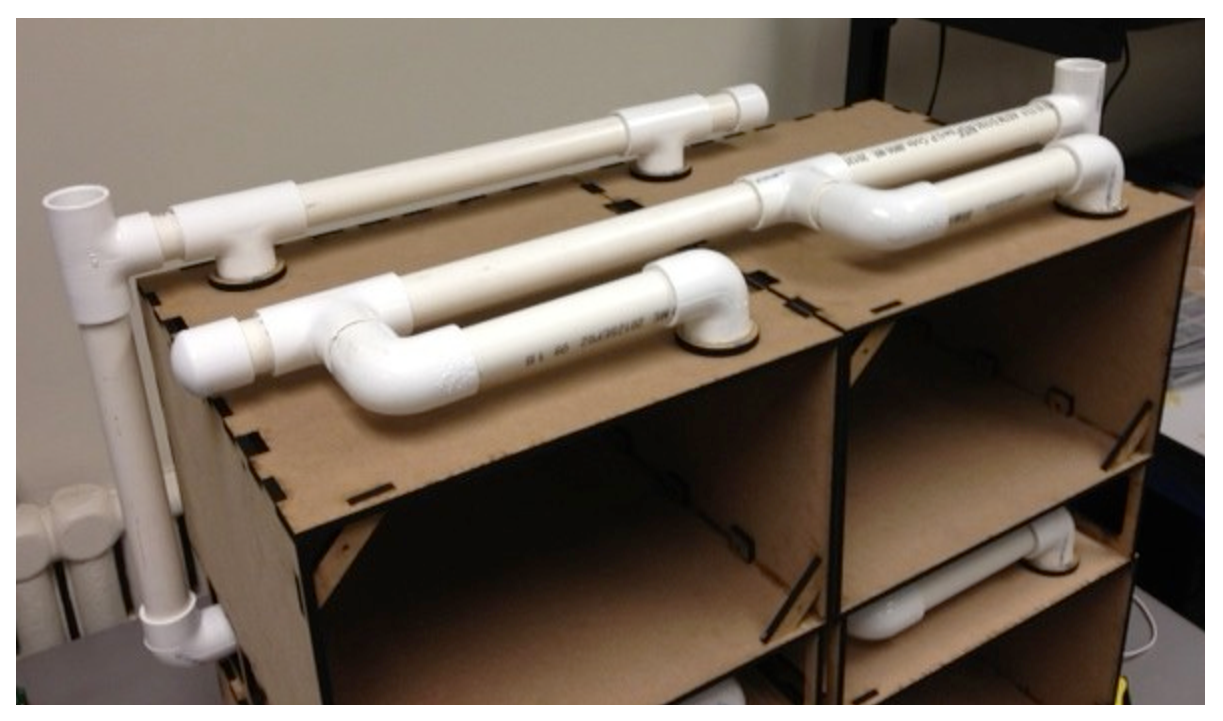
\epsfig{file=ductwork.eps,width=0.8\linewidth,clip=}
\caption{Ductwork Overview}
\label{ductwork}
\end{figure}

\begin{figure}[t]
\centering
\epsfig{file=vav.eps,width=0.8\linewidth,clip=}
\caption{VAV Control with Servo Valve}
\label{vav}
\end{figure}

\emph{Valve Design:}
The use of valves has significant effects on the working of our system.  They not only determine how much air needs to be passed into each room but also enable us to script advanced lazy  schedulers to minimize peak energy consumption by the system as a whole.  The valves were also laser cut and press fit with a combination of quarter-inch and eighth-inch MDF. We also put in a stopper to prevent any leakage when the valve is closed.  We make use of position servo-controlled custom built valves for this HVAC modelling system. There is one valve per room at the inlet and one each at the HVAC outlets. Since cooling and heating are the main tasks of any HVAC system, we designed a single-servo controlled double valve kept at a 90 degree offset to each other which ensured that our system was either cooling or heating at any given time.

\emph{Heating:}
We made use of a 12V hair dryer, shown in \ref{heater}, as our heating element for this test-bed. The output from one point of the double valve behaves as the input to the hair dryer which uses this air to blow over the heating coils and transfer heat to our system. This heated air is sucked in by our supply blower and sent in to the two zones and hence four rooms based on the temperature levels at the HVAC unit. Through experimentation, we realized that the heater would keep rising beyond 65 degree celsius. This is a potential safety concern and hence we limited this range in code to stay within 37 and 40 degree celsius.

\begin{figure}[t]
\centering
\epsfig{file=heater.eps,width=0.8\linewidth,clip=}
\caption{Heater}
\label{heater}
\end{figure}

\begin{figure}[b]
\centering
\epsfig{file=cooler.eps,width=0.8\linewidth,clip=}
\caption{Cooling Box with Copper Coil}
\label{cooler}
\end{figure}

\emph{Cooling:}
One of the main goals of designing such a scaled down version of an actual building with desired variable temperature is the cooling system. While hacking a refrigerator to make use of the compressor and related cooling elements would yield a much larger temperature difference, we decided to use a more conventional approach with a ‘bucket-of-ice’ seen in \ref{cooler}. In essence, we used a 13.5" by 11" by 11" styrofoam box with a 2 foot long half-inch diameter copper tube submerged in cubes of ice. With the other output point of the double valve open, we could circulate cool air in to the rooms using the same supply blower. We saw temperature drops of 5 to 6 degree celsius. This drop in temperature is very realistic but in order to monitor faster dynamics, we decided to build an enclosure for the entire system, excluding the cooling box.

\emph{Enclosure:}
Due to the large size and various number of linkages in the entire system, there would still be some leakage and this would affect the dynamics of the system in a very slow and realistic manner. But since this is meant to be a test bed we need to be able to implement algorithms and see the results as soon as possible. This is the primary purpose of the enclosure, which can be seen in \ref{encl}, to help accelerate our simulations on EnRoute 2.0. The enclosure measures 38.5" by 42.5" by 20" and is designed for minimum raw material requirements. This means that we made a frame out of MDF and the view window out of two 16" by 32" clear acrylic sheets. To simulate natural heating in a building due to the sun, we decided to use an incandescent bulb. Since the dimensions of the enclosure exceed the workspace limits of the laser, we cut and built the enclosure using conventional power tools.

\begin{figure}[t]
\centering
\epsfig{file=encl.eps,width=0.8\linewidth,clip=}
\caption{Enclosure Design}
\label{encl}
\end{figure}

\begin{center}
{\bf Electronics}
\end{center}

As mentioned earlier, valves in every room are controlled by small servo motors. These servo motors, shown in \ref{servo}, are position servo motors controlled using the PWM pins on the mBed. Each valve is controlled separately by a servo motor.  The servo motor that we used can be found here (https://www.sparkfun.com/products/9064).    

The temperature sensors \ref{temp} that we use are TMP-36. This sensor is inexpensive and provides an analog voltage based on the ambient temperature and so were connected to the mBed using ADC input pins. This sensor can be found from (https://www.sparkfun.com/products/10988?).  We placed one temperature sensor in each zone, one outside the zones but inside the enclosure, and one in the supply air duct 

We use a total of 3 blowers, as shown here \ref{blower}, to force air through the ductwork.  These blowers can be found at (https://www.sparkfun.com/products/11270).  This blower provides in excess of 12 CFM of flow at 1A of rated current, which worked well for us.  The forward blower pulls air from the heater or cooler and delivers it to the ductwork. The return blower is used to suck the air out from each zone and the third valve was used to pass air from the return valve to either the heater or cooler.

\begin{figure}[t] 
	\centering
        \begin{subfigure}[l]{0.4\columnwidth}
		\centering
		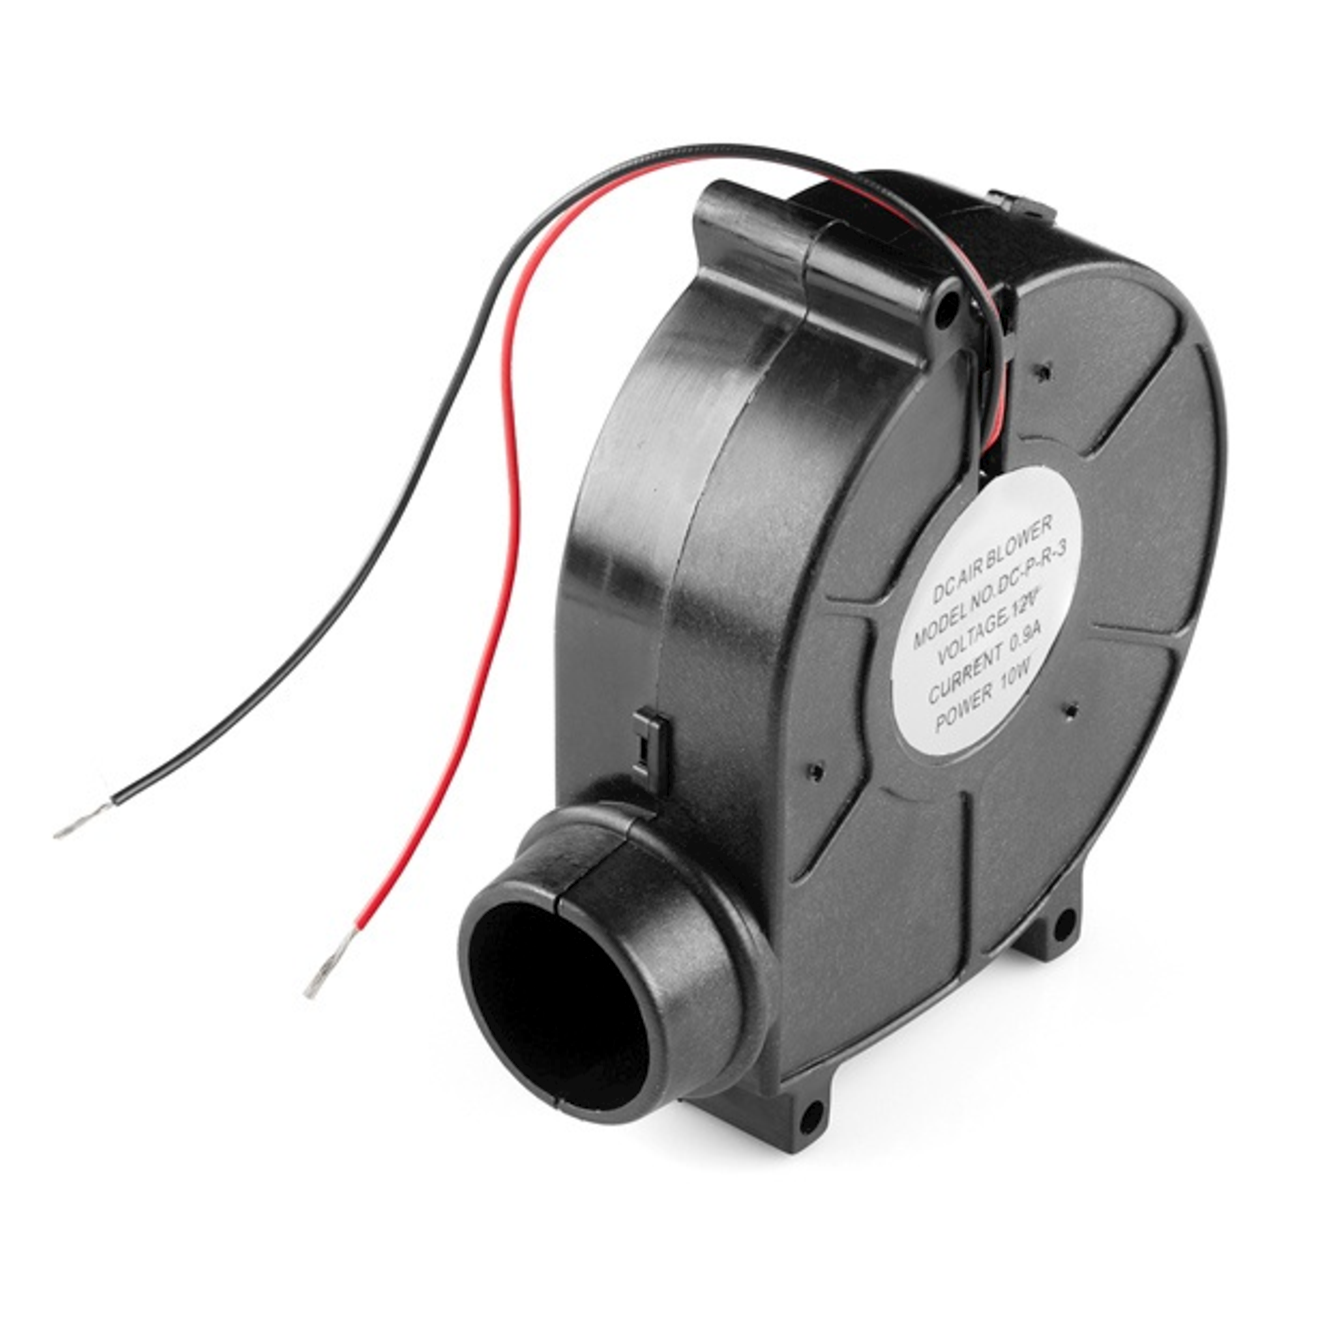
\epsfig{file=blower.eps,width=1\linewidth,clip=}
		\caption{Blower}
		\label{blower}
        \end{subfigure}
        \begin{subfigure}[r]{0.4\columnwidth}
		\centering
		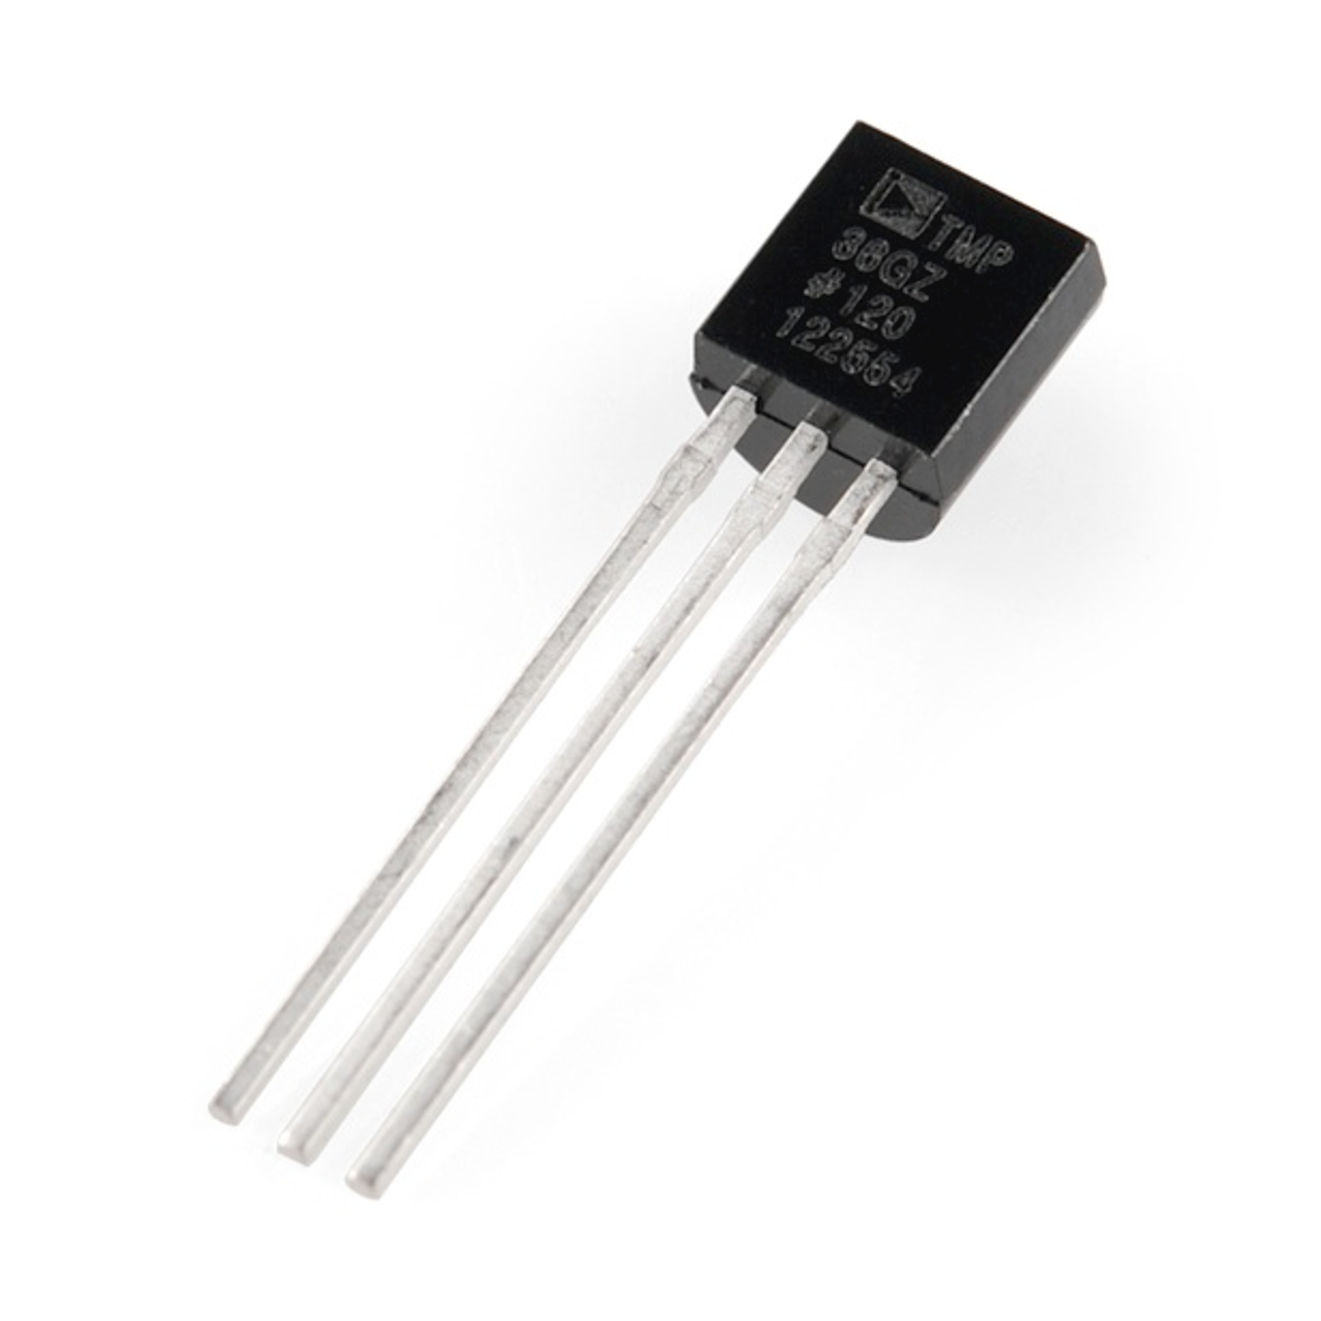
\epsfig{file=temp.eps,width=\linewidth,clip=}
		\caption{Temp Sensor}
		\label{temp}
        \end{subfigure}
	\\
        \begin{subfigure}[r]{0.4\columnwidth}
		\centering
		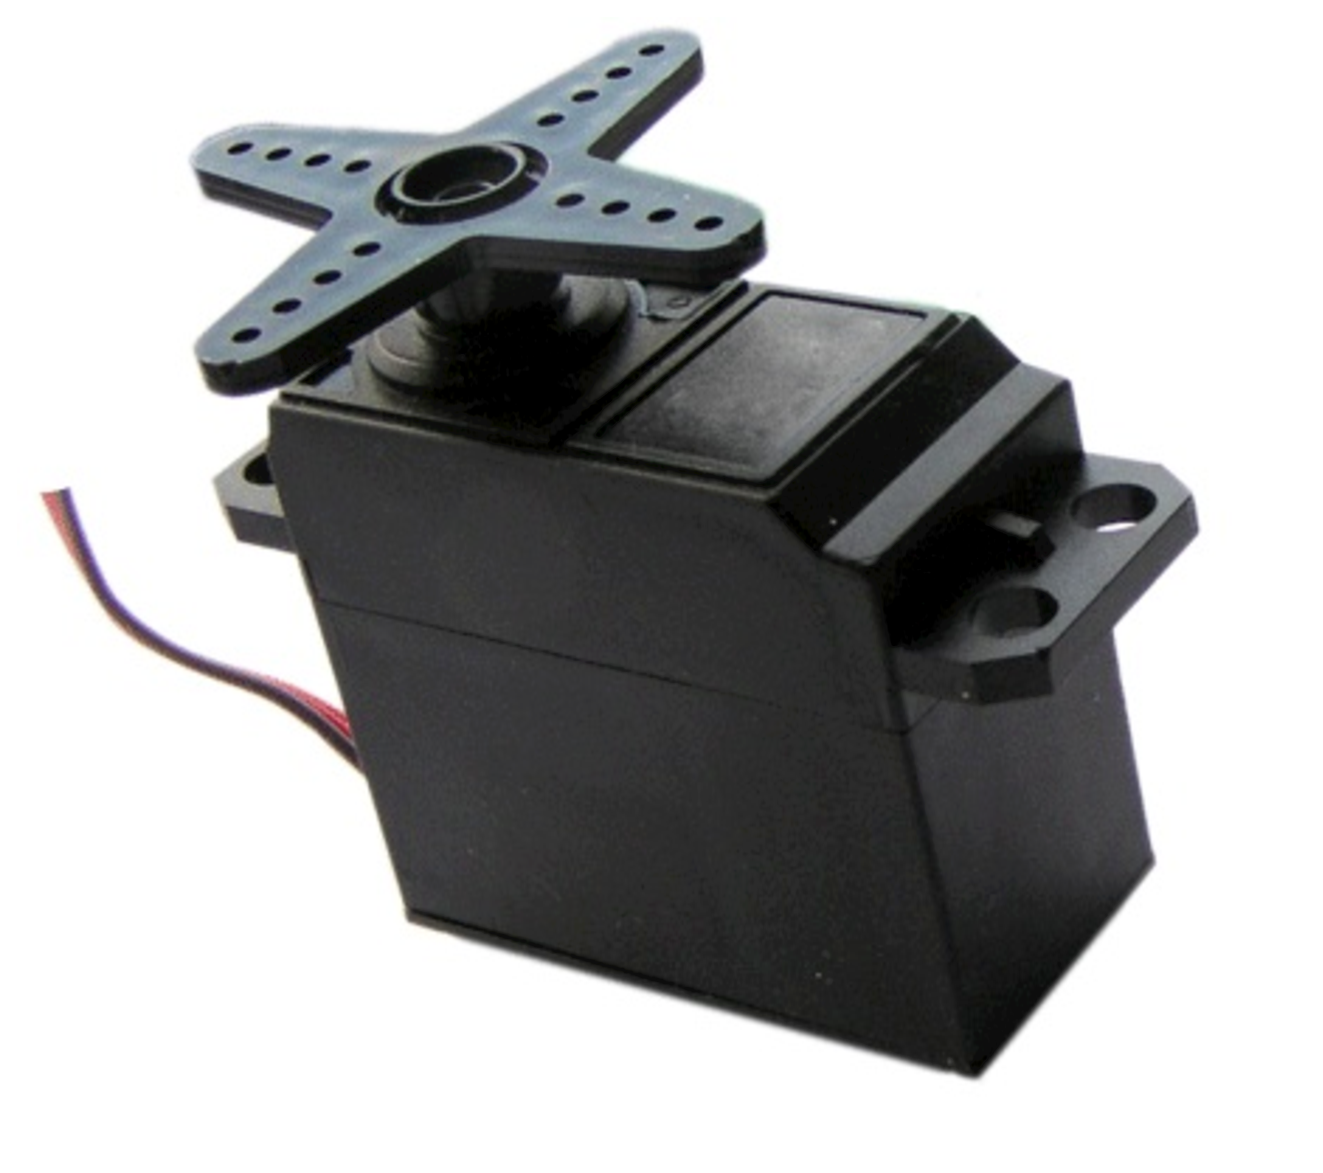
\epsfig{file=servo.eps,width=0.8\linewidth,clip=}
		\caption{Servo}
		\label{servo}
        \end{subfigure}
	\caption{Electronics}
        \label{electronics}
	\vspace{-7mm}
\end{figure}

\begin{figure}[b!]
\centering
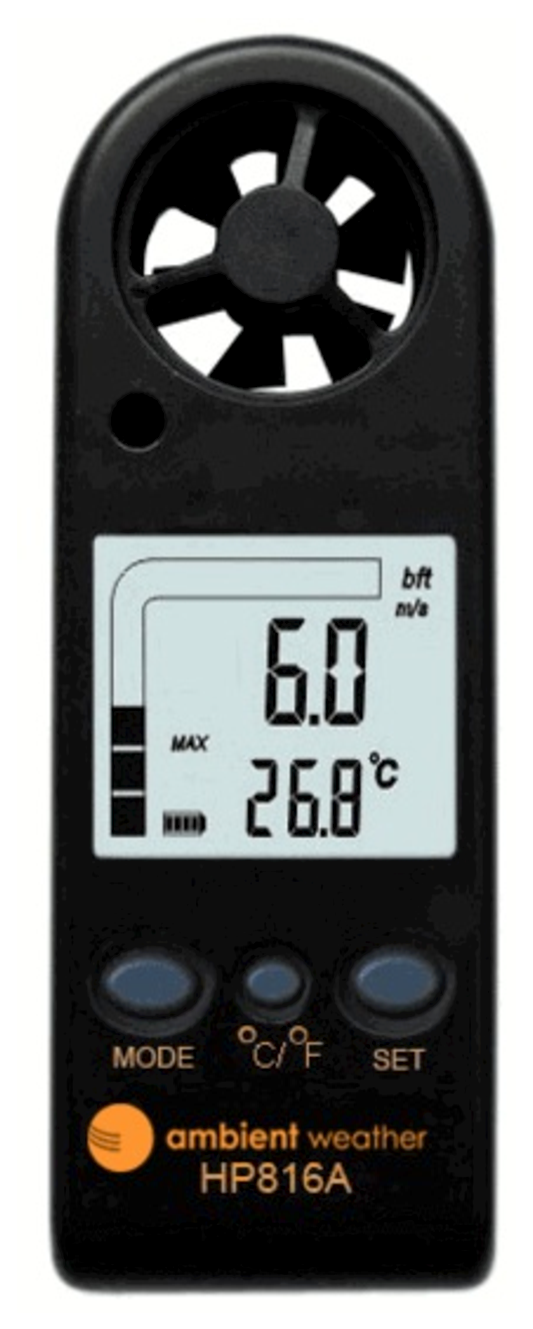
\epsfig{file=flow.eps,width=0.3\linewidth,height=0.7\linewidth,clip=}
\caption{Flow Meter}
\label{flow}
\end{figure}

These blowers need a 12V supply, so we use the SN754410 H-Bridge to produce a 12V signal from a 5V PWM input signal supplied from the mBed.  These H-Bridge circuits are rated for up to 1A continual current draw which is the maximum our blowers are rated for.

We use air flow meters, displayed here \ref{flow}, from Ambient Weather (http://www.ambientweather.com/amhp816a.html) to measure the speed at which air is entering the zones as well as the airflow near the forward valves. Speed data is then converted to volumetric flow rate in CFM (cubic feet per minute) for displaying in the GUI.

\begin{center}
{\bf Software}
\end{center}

Software for this project is implemented both on mBed microcontrollers, which are the nodes physically interfaced with the test-bed, and in MATLAB, which acts as the master planner of the system by gathering all data and calculating the control outputs for the servo valves and blower states.  The system architecture for our system can be seen here \ref{sys_arch}.

\begin{figure}[b!]
\centering
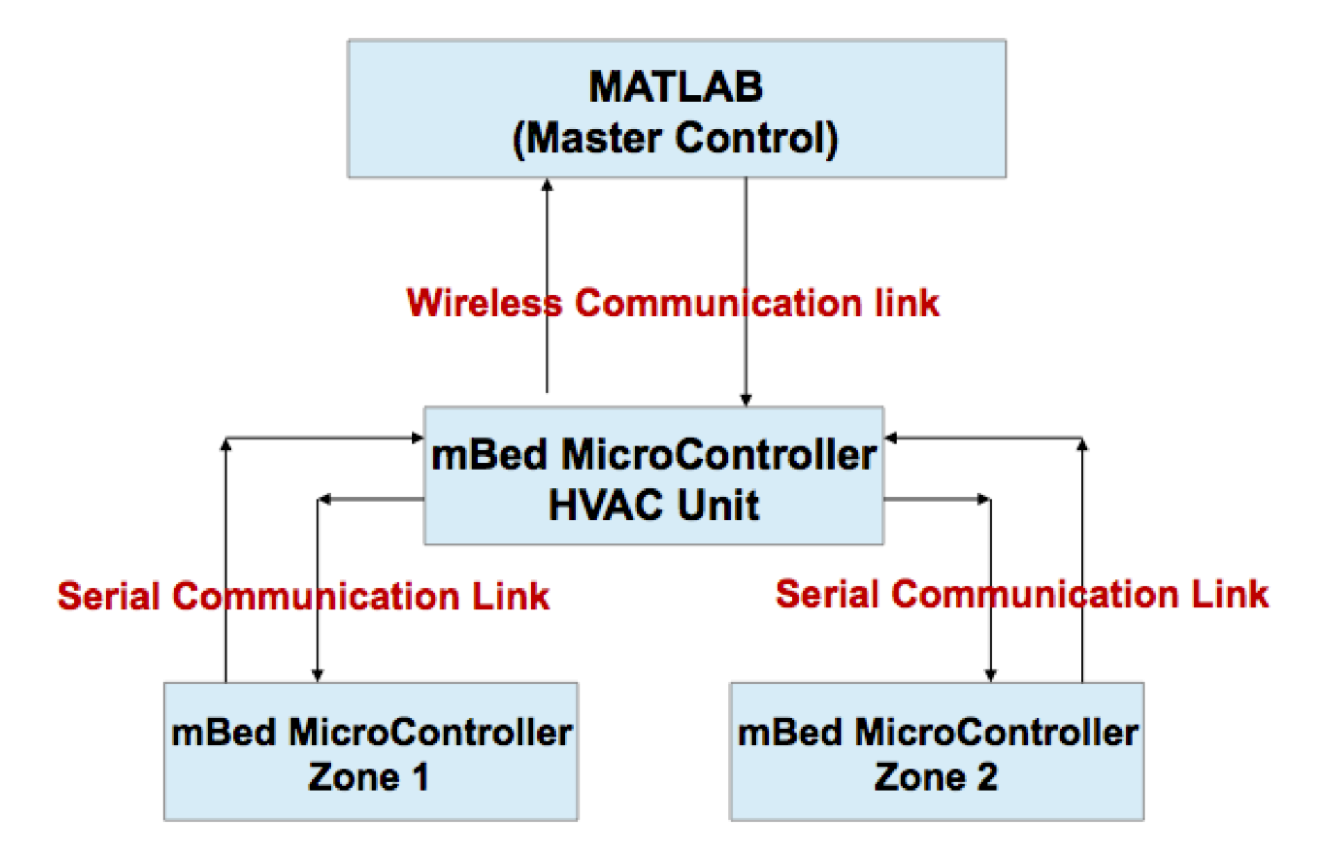
\epsfig{file=sys_arch.eps,width=\linewidth,clip=}
\caption{System Architecture}
\label{sys_arch}
\end{figure}

The system utilizes three mBeds:  one for the lower zone that controls rooms 3 and 4, one for the upper zone that controls rooms 1 and 2, and one for the HVAC and AHU system.  The mBeds placed in each zone gather and interpret data from temperature sensors and flow meters, relay this data to the HVAC mBed over RS232 protocol, and subsequently receive control data from the HVAC mBed which defines how the servo position should be set.  The HVAC mBed also reads from two temperature sensors and a single flow meter, then requests and receives data from the two zone mBeds subsequently, and transmits all data to the host PC.  Additionally, data returned from the PC instructs the HVAC mBed how to control the recycle air valves and AHU blowers.

Within MATLAB a front-end GUI has been created which allows the user to view all data from the test-bed, in real time while the simulation is running, and control all controllable devices (servo valves, heating or cooling, and blowers).  The Overview tab, shown here in \ref{overview_tab}, displays all data from the four rooms and provides a means for manual control over the servo valve for each zone.  Additionally, there are tabs which display all data simultaneously for each room.  The HVAC tab, shown in \ref{HVAC_tab}, allows control of the recycle air valves and blower states.  Also, data is plotted for all HVAC devices including a current sensor monitoring the supply blower.  Finally, the Control tab provides the user a way to control all aspects of the system including room set points, control algorithms, serial port, IP address (see below), whether the system is heating or cooling, and several other features.  This tab is shown in \ref{control_tab}.  

\begin{figure*}[t]
\centering
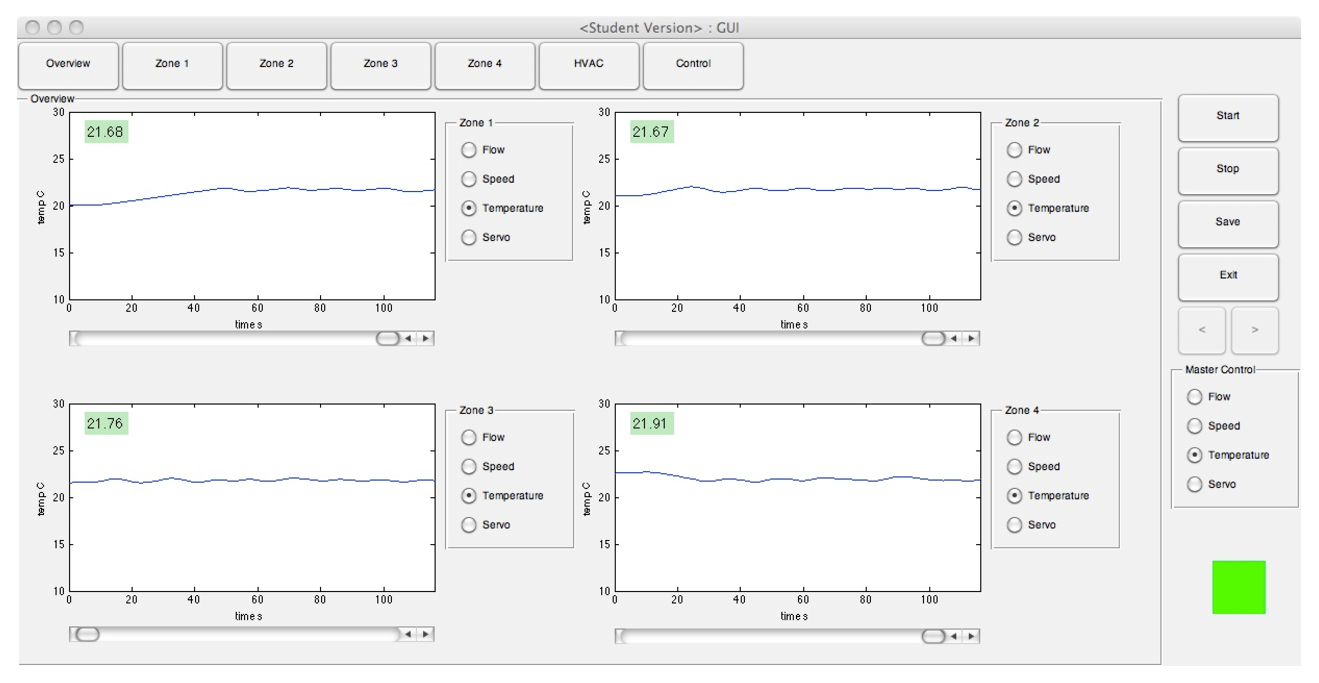
\epsfig{file=overview_tab.eps,width=\linewidth,clip=}
\caption{Dashboard Overview Tab}
\label{overview_tab}
\end{figure*}

\begin{figure*}[b!]
\centering
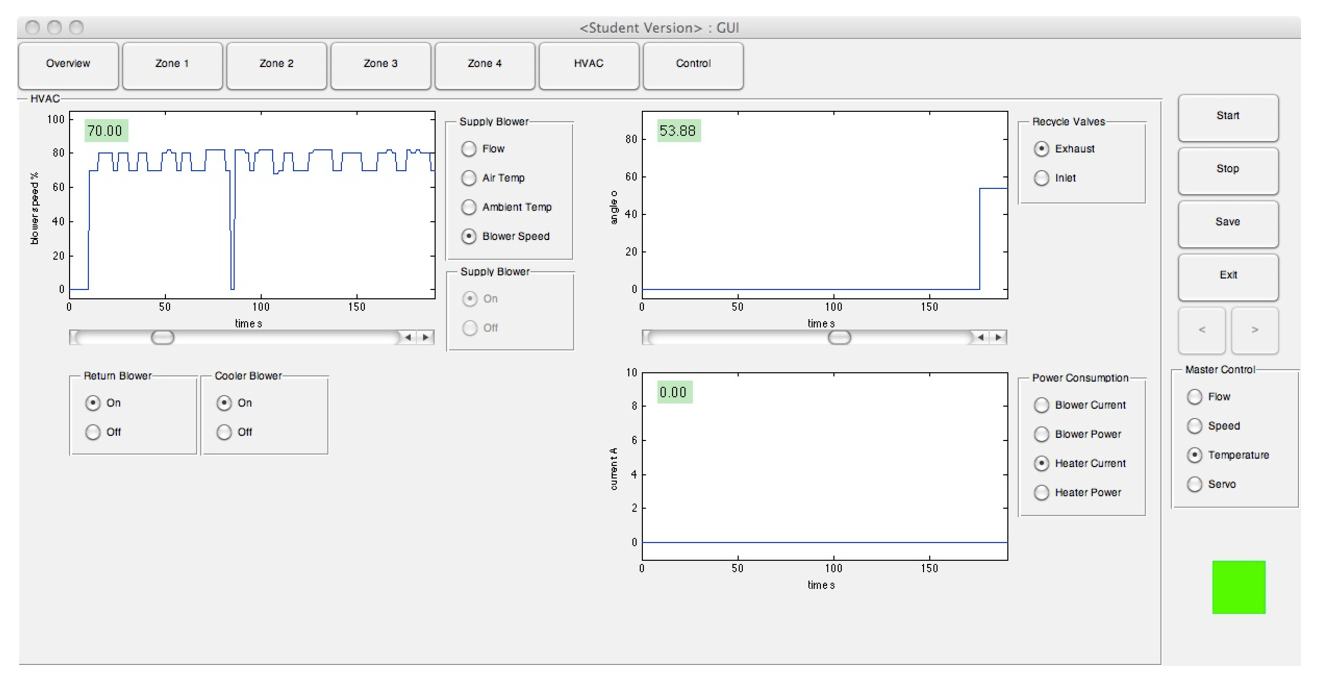
\epsfig{file=HVAC_tab.eps,width=\linewidth,clip=}
\caption{Dashboard HVAC Tab}
\label{HVAC_tab}
\end{figure*}

\begin{figure*}[t]
\centering
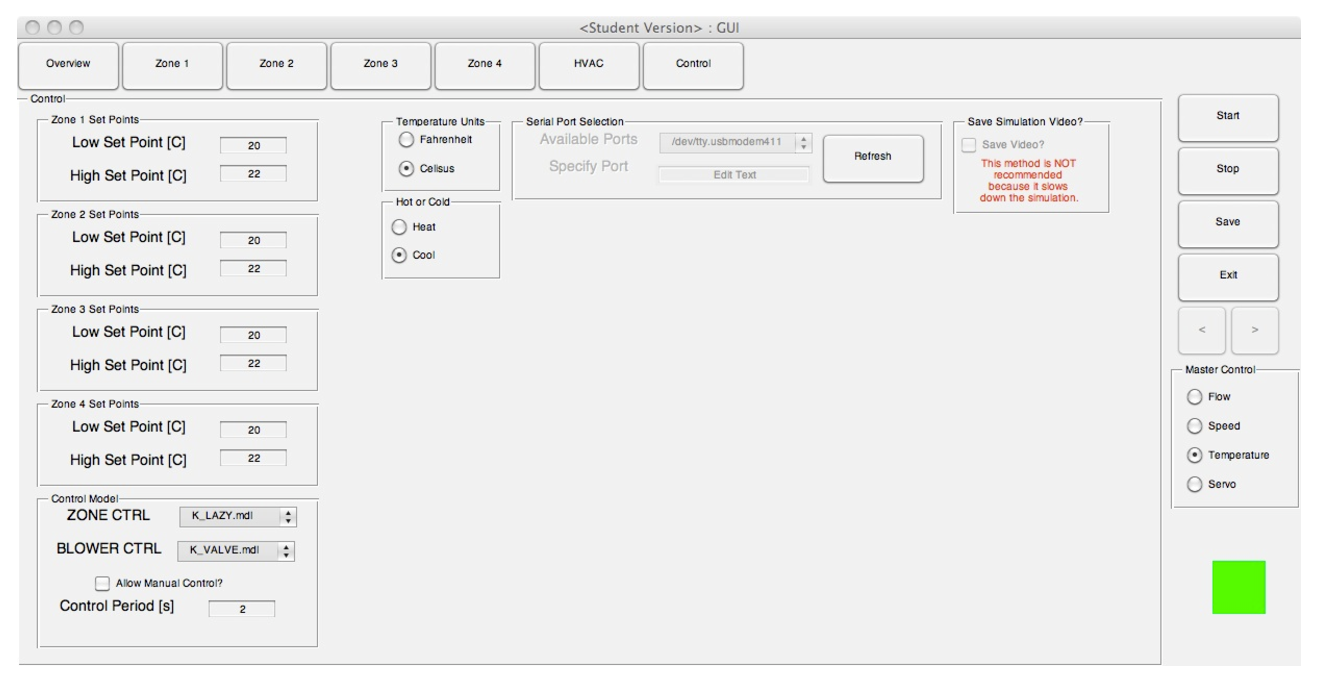
\epsfig{file=control_tab.eps,width=\linewidth,clip=}
\caption{Dashboard Control Tab}
\label{control_tab}
\end{figure*}

In order to have the test-bed be controlled from virtually anywhere in the world we decided to incorporate IP-IP communication. The mBed inherently supports Ethernet, so we realized a UDP server on the mBed and our MATLAB GUI acted as the UDP client. The client (MATLAB) sends a packet to the server (mBed) requesting data. The mBed then parses the packet which contains instructions as per the user’s input. The mBed, at the same time, also collects data such as the temperature, flow rate, and servo motor position, passing it back to the client as a UDP packet.

\begin{figure}[t]
\centering
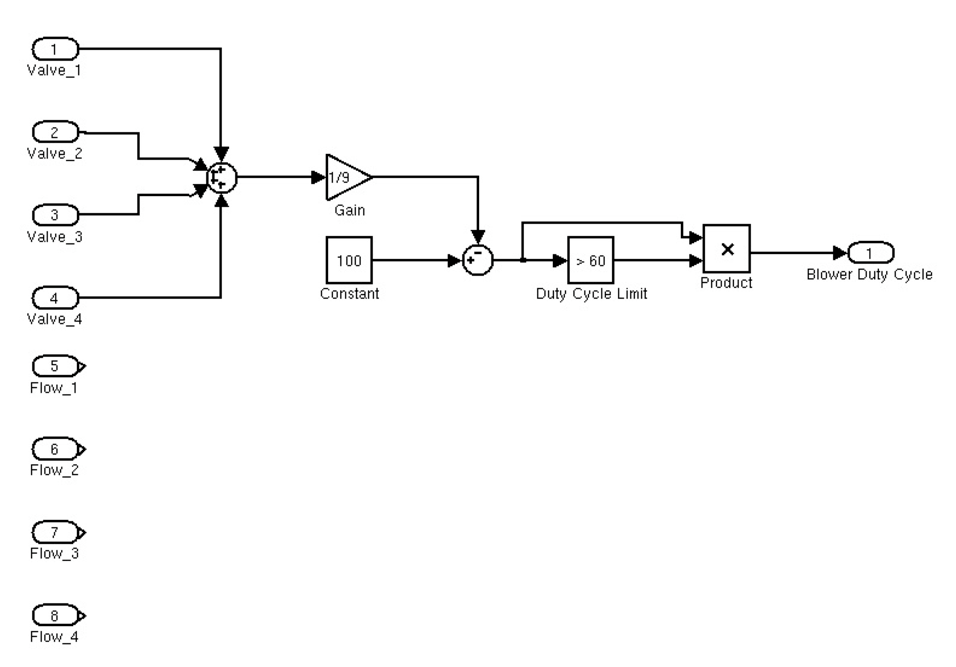
\epsfig{file=blower_mdl.eps,width=\linewidth,clip=}
\caption{Blower Control Model}
\label{blower_mdl}
\vspace{-5mm}
\end{figure}

Additionally, since not all those interested in testing algorithms are intimately familiar with MATLAB programming, the system will accept control algorithms designed in MATLAB as long as they follow a basic template design.  For example, the blower control model MUST have eight total inputs (four for valve position and four for flow meters, in this order) and a single output which defines the percent of max power supplied to the blower.  An example model may be seen in \ref{blower_mdl}.  If the user wishes to define more inputs (in the form of constants), a single initialization file can be edited to load the inputs at the beginning of the control loop.  This is best done for inputs that do not change (such as set points).  An example of such a case can be seen in \ref{lazy}, which has constant inputs for set points and control limits for the lazy scheduler.

\begin{figure}\centering
        \begin{subfigure}[t]{\linewidth}
                \centering
                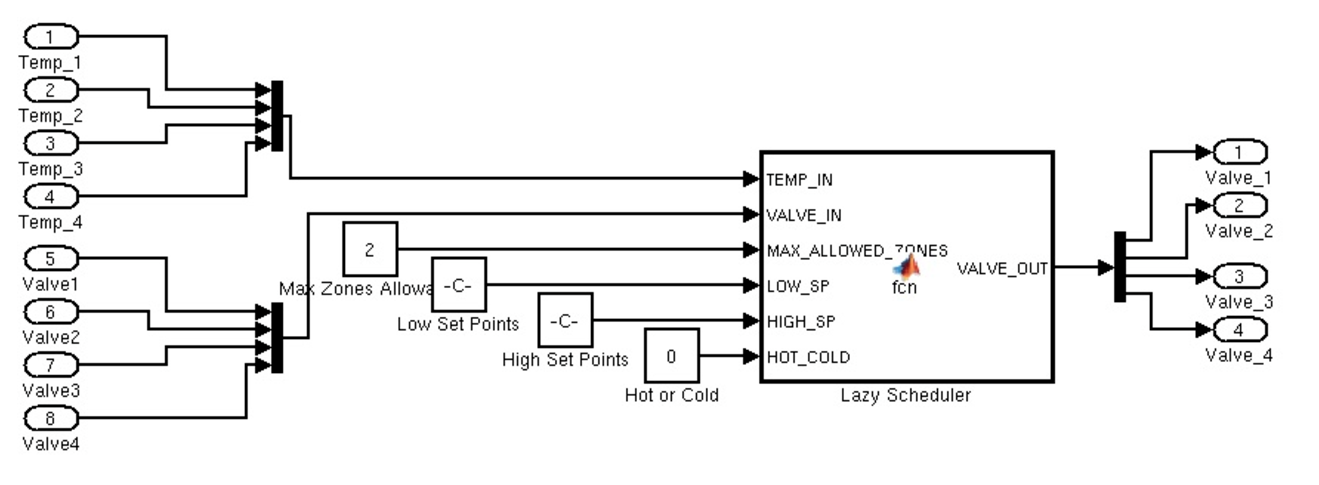
\includegraphics[width=\linewidth]{lazy_mdl}
                \caption{Lazy Scheduler Model}
                \label{lazy_mdl}
        \end{subfigure}
	\\
        \begin{subfigure}[b]{\linewidth}
                \centering
                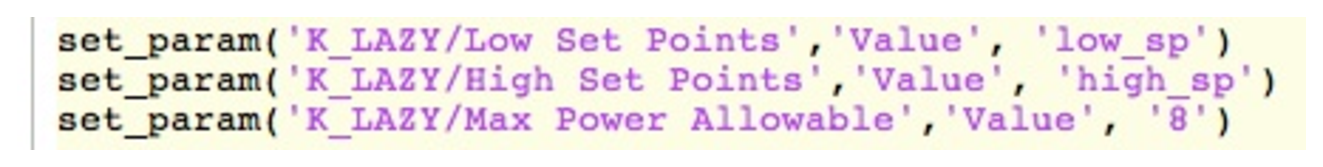
\includegraphics[width=\linewidth]{lazy_code}
                \caption{Code Sample for Model Initializer}
                \label{lazy_code}
        \end{subfigure}
        \caption{More Advanced Model w/ Constant Inputs}\label{lazy}
\end{figure}

\begin{center}
{\bf Use as a Test-Bed}
\end{center}

With our custom designed front-end system in MATLAB interfaced with our main mBed controller, we control the working of the test bed. The control could be manual from the user or from a Simulink model fed in by the user. This is one of the key advantages of our test bed where a user with minimal experience can put in a simple simulink model and let our system simulate the results.

As mentioned earlier, the AHU is the main component of any HVAC system. We used 3 blowers for this purpose. When we triggered the supply blower, based on the mode (cooling or heating) selected, the room temperatures would vary accordingly. Further temperature variations were seen based on the angle of the corresponding room valves that were also controlled from our GUI. These valve angles were determined based on the temperature requirements of the room under question. It is imperative for an energy efficient system to adjust the amount of air pumped in based on the requirements of the room i.e if a valve to a room is closed, it doesn’t make sense in supplying the same amount of air for the other 3 rooms especially if those rooms don’t need it. This is where the lazy scheduler plays a big role in determining efficient energy utilization throughout the entire piping.  

A very useful feature we incorporated into this revision of EnRoute is the ability to remotely do all of the above and not be tethered to the system during operation.  We achieved this over the internet using dedicated IPs for viewing and controlling the system.

\begin{center}
{\bf Simulation Results}
\end{center}

The simplest algorithm for testing is a pure ON-OFF controller that will keep all zones oscillating between their high and low set points with no regard to total simultaneous power consumption.  Using this type of test we can confirm that the systems are functioning as they should as well as gain an understanding of the dynamics for the rooms.  These simulations were run using the heating aspect of the system which requires control of the outlet air temperature.  If the heater were left unconstrained it would quickly become too hot and would damage the system; therefore, the mBed limits the heater output temperature to within a small acceptable range.  Using this heater output we have implemented an ON-OFF controller whose simulation results for Room 1 are shown in \ref{on_off_rm1_temp} and the total blower power during the simulation is shown in \ref{on_off_blower}.  It is worth noting that the blower is constrained to operate in the 60\% to 100\% range.

\begin{figure}[t]
\centering
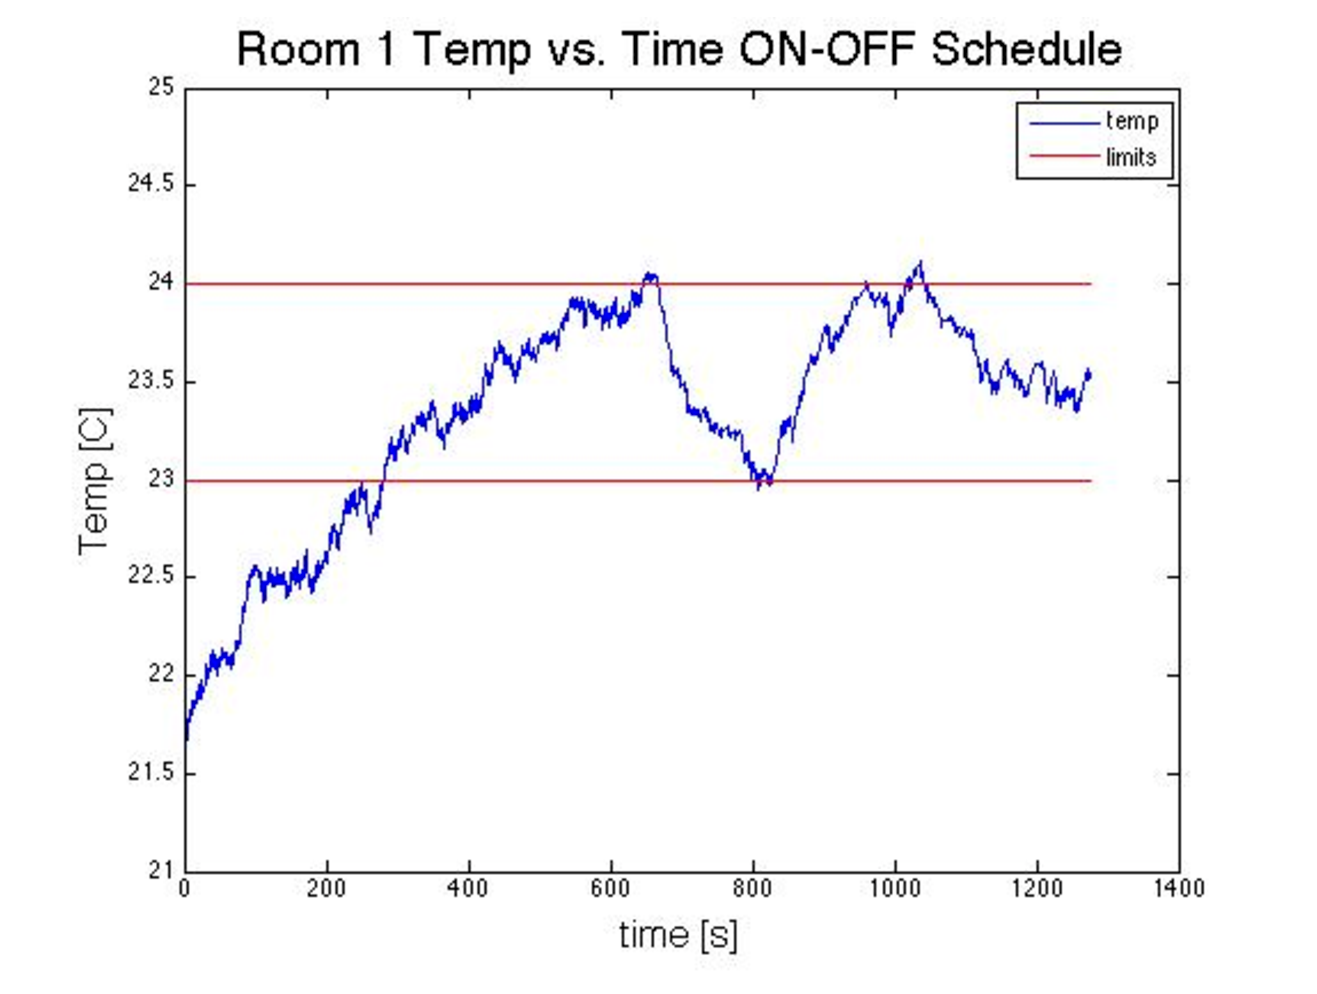
\epsfig{file=on_off_rm1_temp.eps,width=\linewidth,clip=}
\caption{Room 1 Temperature Response to On-Off Control}
\label{on_off_rm1_temp}
\end{figure}

\begin{figure}[t]
\centering
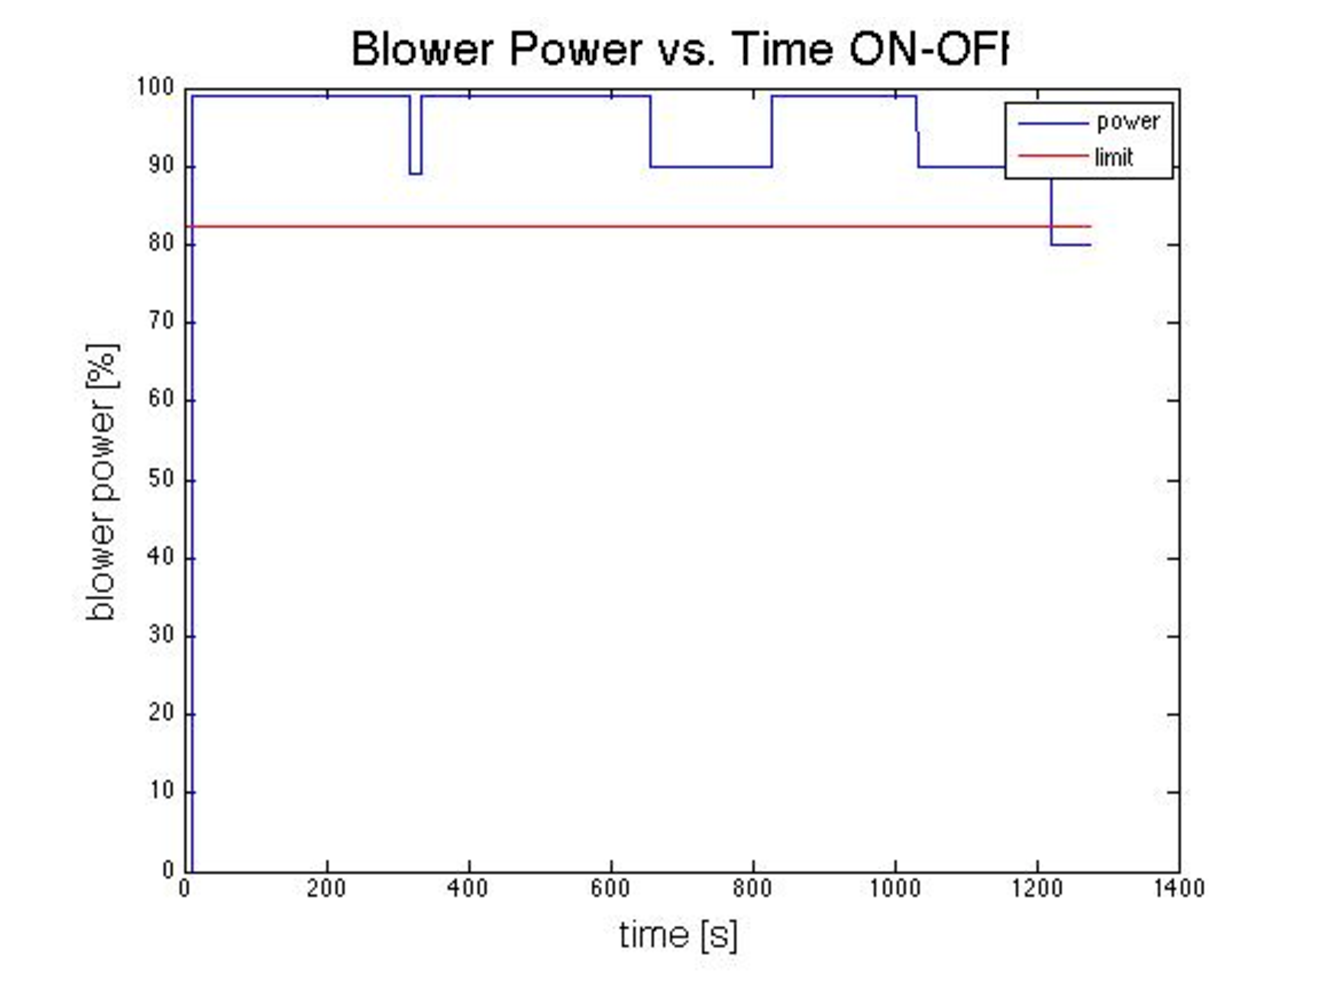
\epsfig{file=on_off_blower.eps,width=\linewidth,clip=}
\caption{Room 1 Temperature Response to On-Off Control}
\label{on_off_blower}
\end{figure}

\begin{figure}[b!]
	\centering
        \begin{subfigure}[t]{\linewidth}
                \centering
                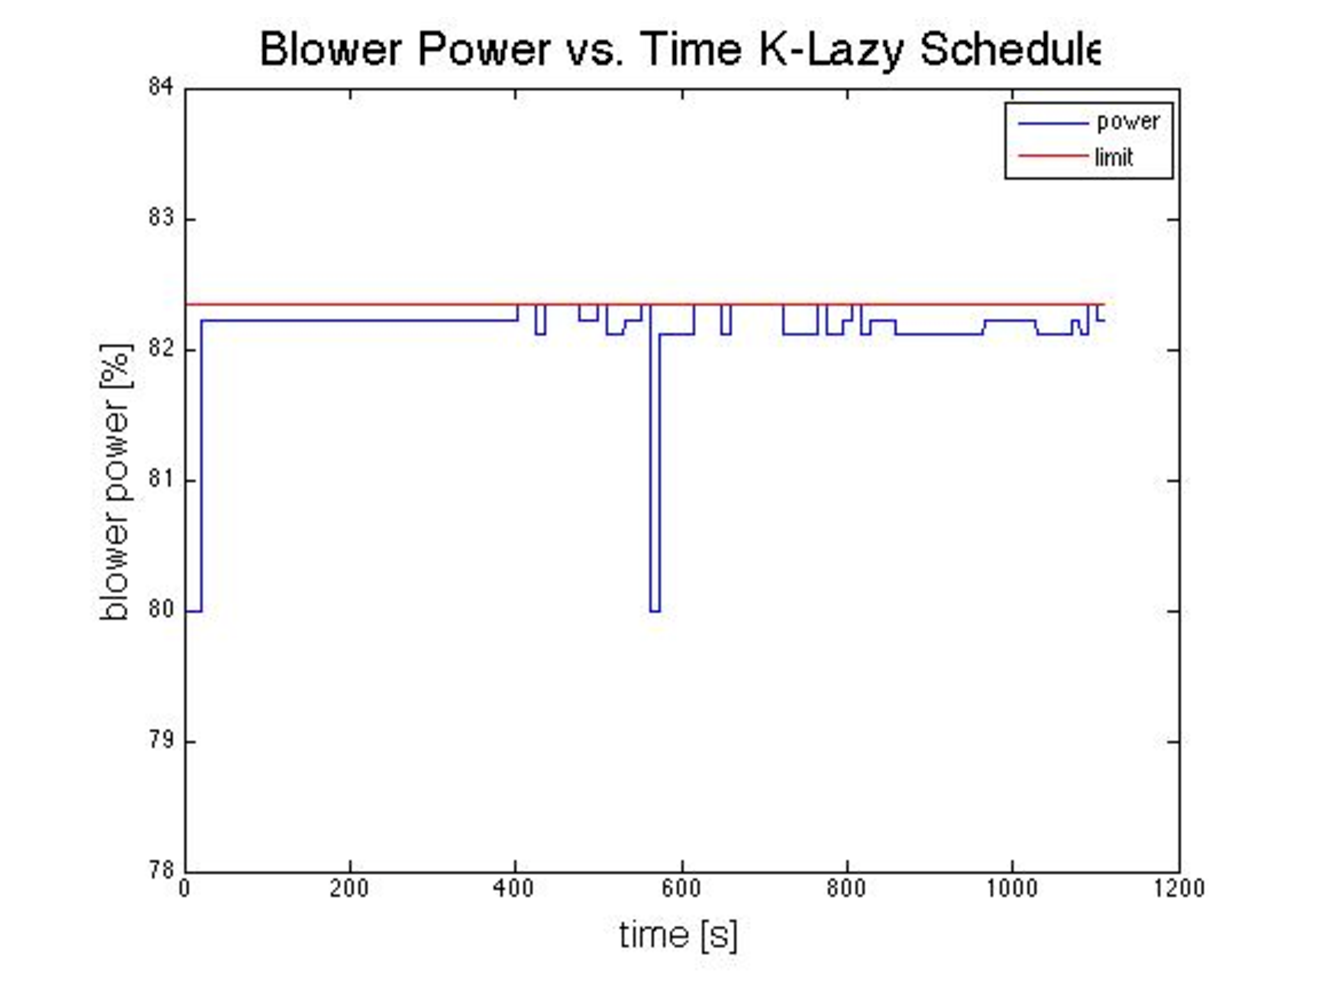
\includegraphics[width=\linewidth]{k_lazy_blower}
                \caption{Lazy Scheduler Blower Output}
                \label{k_lazy_blower}
        \end{subfigure}
	\\
        \begin{subfigure}[b]{\linewidth}
                \centering
                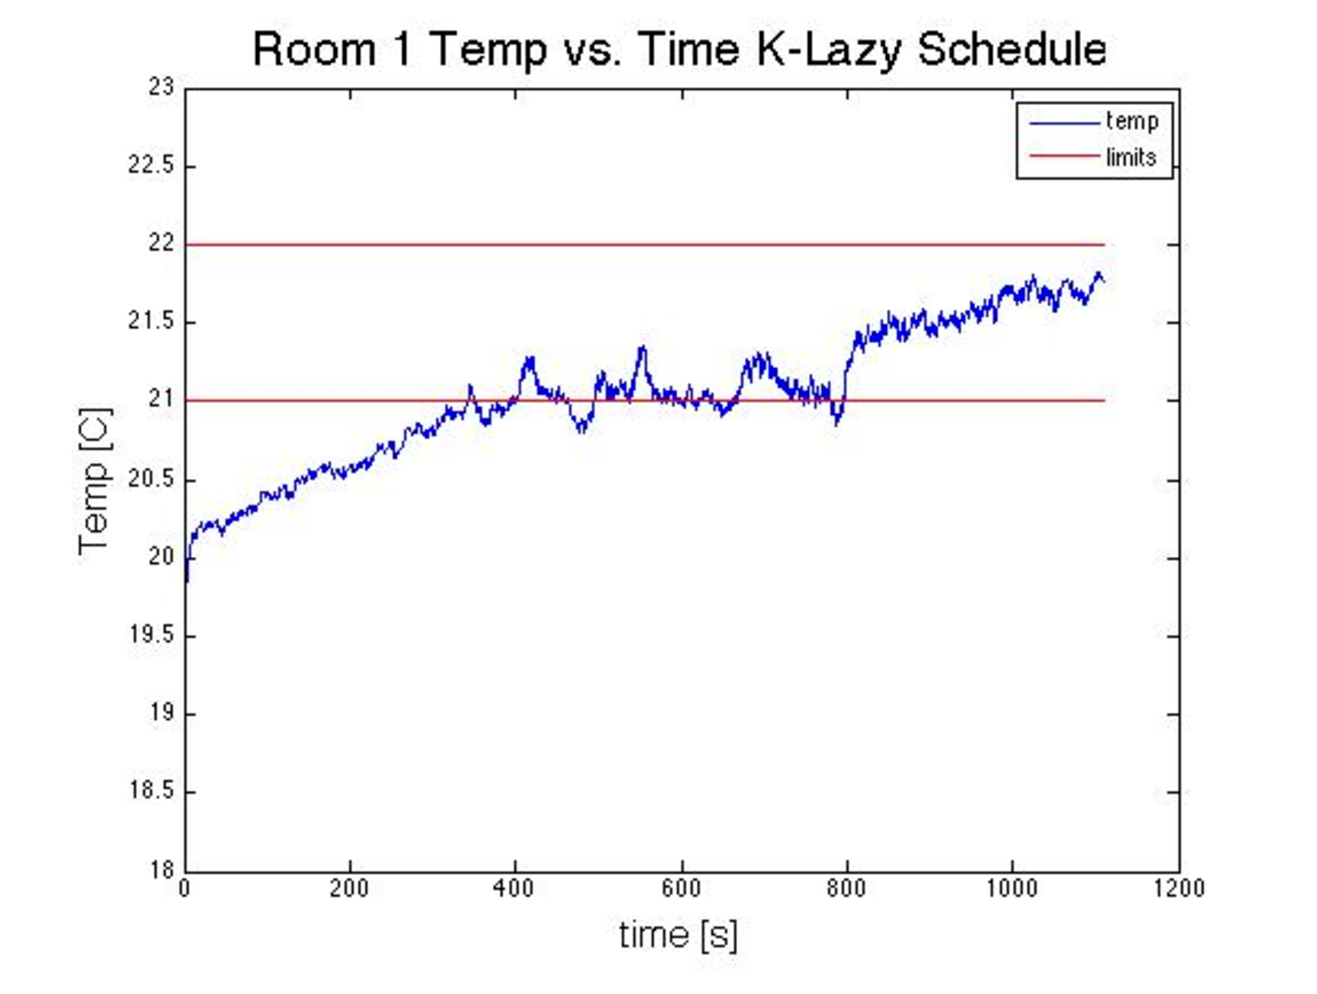
\includegraphics[width=\linewidth]{k_lazy_rm1_temp}
                \caption{Room 1 Temperature Response Lazy Scheduler}
                \label{k_lazy_rm1_temp}
        \end{subfigure}
	\\
        \begin{subfigure}[b]{\linewidth}
                \centering
                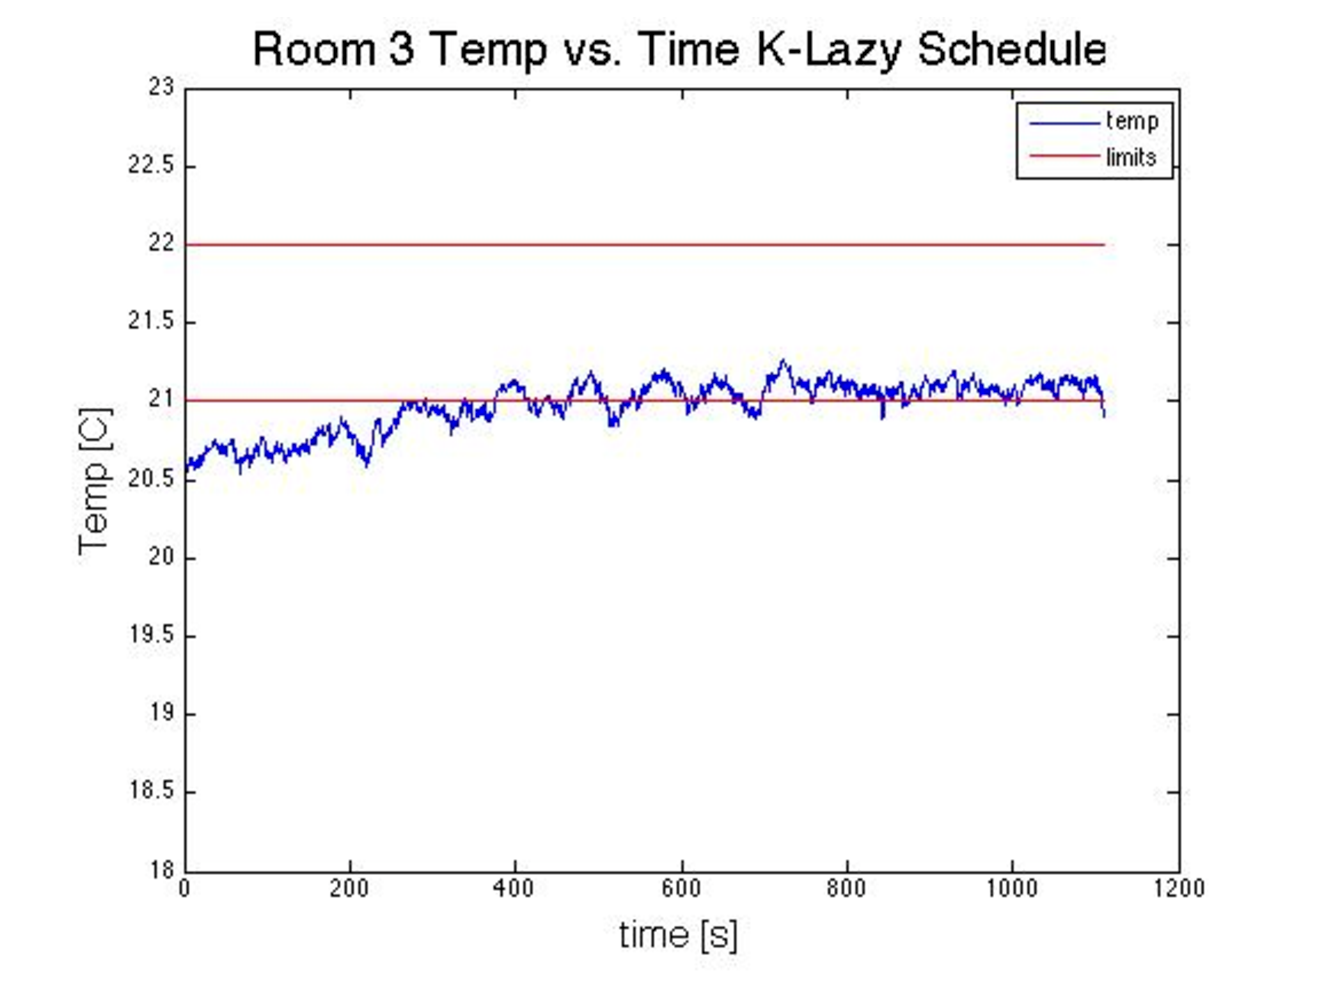
\includegraphics[width=\linewidth]{k_lazy_rm3_temp}
                \caption{Room 3 Temperature Response Lazy Scheduler}
                \label{k_lazy_rm3_temp}
        \end{subfigure}

        \caption{Lazy Scheduler Simulation}\label{lazy_sim}
\end{figure}

For further testing of our system we implemented a basic lazy scheduler algorithm.  A lazy scheduling algorithm only makes intelligent decisions when a room reaches a threshold point by either closing the air flow to the room or setting the room as critical.  Simulation results for this test are shown in \ref{lazy_sim} and \ref{lazy_sim_valve}.

\begin{figure}[t]
	\centering
        \begin{subfigure}[b]{\linewidth}
                \centering
                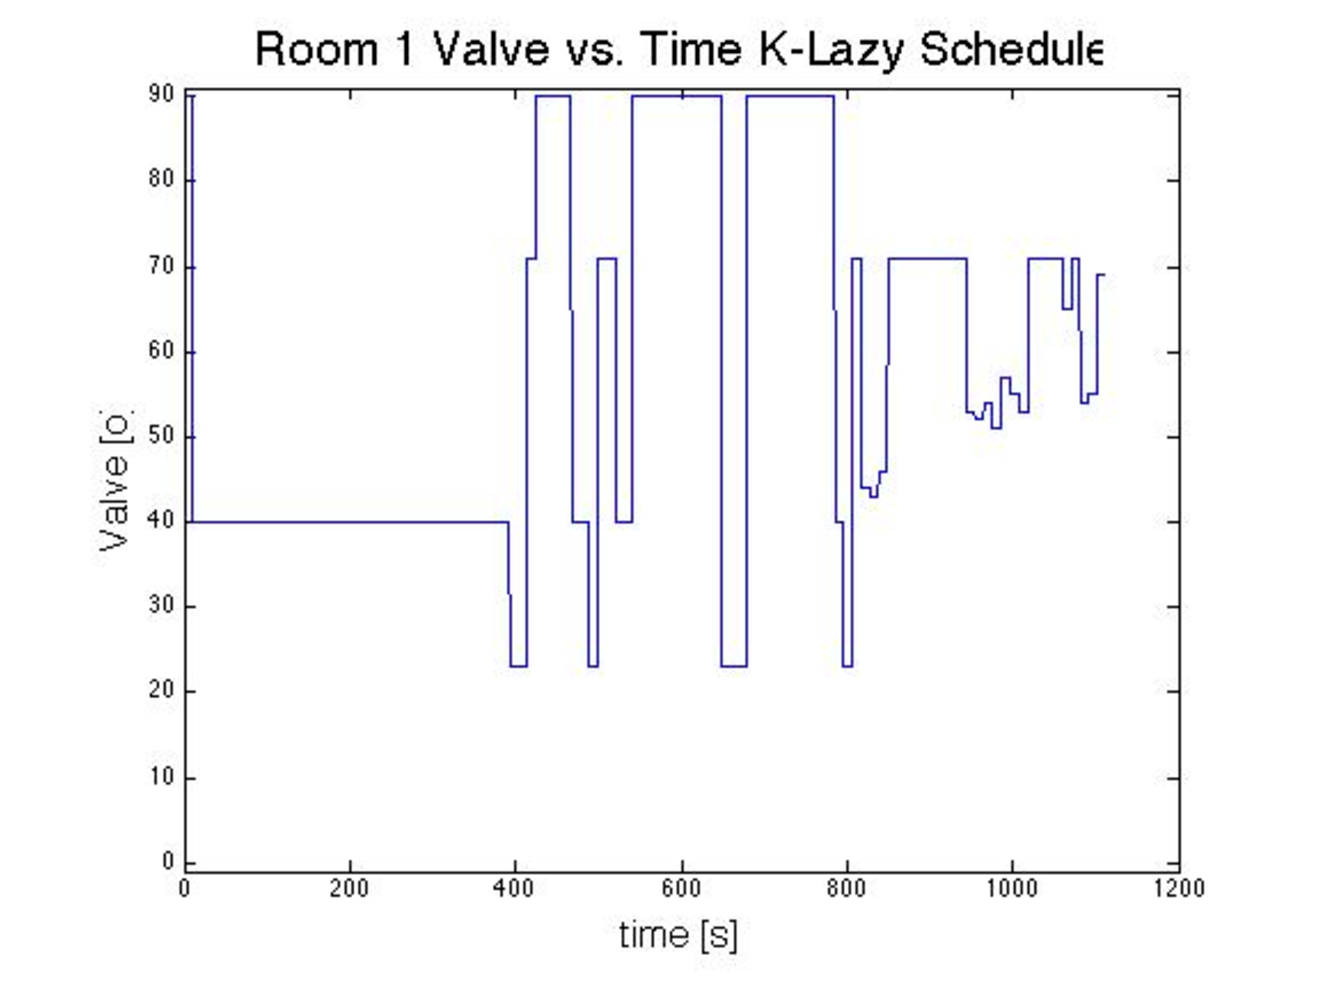
\includegraphics[width=\linewidth]{k_lazy_rm1_valve}
                \caption{Room 1 Valve Response Lazy Scheduler}
                \label{k_lazy_rm1_valve}
        \end{subfigure}
	\\
        \begin{subfigure}[b]{\linewidth}
                \centering
                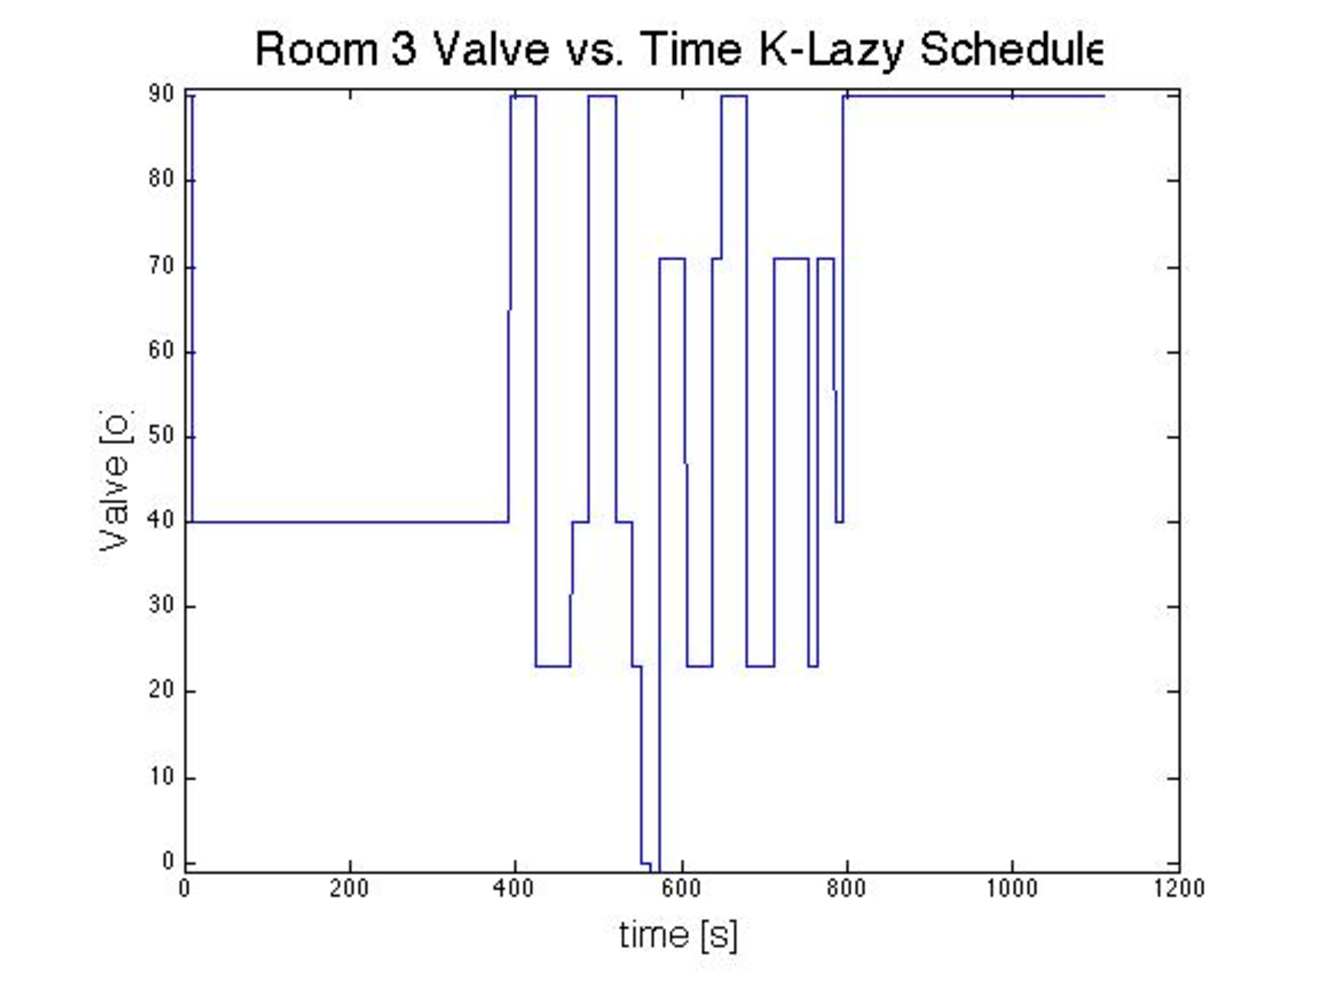
\includegraphics[width=\linewidth]{k_lazy_rm3_valve}
                \caption{Room 3 Temperature Response Lazy Scheduler}
                \label{k_lazy_rm3_valve}
        \end{subfigure}
        \caption{Lazy Scheduler Simulation}\label{lazy_sim_valve}
\end{figure}

The goal of this project was not to design sophisticated test algorithms for furthering research into energy scheduling, it was to design a test-bed so that others may develop algorithms and test them independently.  Therefore, little time was spent designing these controls and more time was focused on building a simple user interface which would allow others to easily load and test their own algorithms.

\begin{center}
{\bf Future Work}
\end{center}

Our list of proposed future work includes the following items:

1.  The ice box worked really well for us giving us a change of 5 deg C, but this change was not realized once the test-bed was assembled. We do realize that the dynamics of the system can be greatly improved if, instead of using a styrofoam box filled with ice as a cooling unit, we use a heat pump of some sort (i.e. the internal workings of a fridge) for the cooling mechanism.  

2.  Currently we have a common heating system for all the zones which makes it difficult for the user to keep test individual dynamics of each zone. We will want to incorporate the ability to control heat into each room individually through the use of some type of local reheat element. This would make our current system more flexible.

3.  Increasing the airflow to each room would improve dynamics and reduce the time to heat and cool each zone.  To achieve this small CPU fans could be added to the inlet of each room.  This requires little hardware work, but will involve more significant software and electronics modifications if the fans should be controllable.

4.  All systems used in real buildings implement a protocol called BACnet to interact with each other. So to take this system one step further towards a realistic system we will want to create a BACnet server on the mBed. In our endeavor to take this system further towards reality we wish to replace our mBeds with real BACnet clients and BACNet servers.

5.  Currently we have tested a bare minimum lazy scheduler as well as a more advanced lazy scheduler. Other algorithms/scheduling policies are something that will be implemented.

\vspace{5mm}

\begin{center}
{\bf Conclusion}
\end{center}

In this project we set out to design a test-bed for remote investigation of control algorithms aimed at green scheduling practices.  With high costs of electricity during peak operating hours, significant savings can be realized through effective control structures designed at limiting the total simultaneous power consumption through a system integration approach.  Our design includes an air handling unit, variable air volume control, ductwork, heating, and cooling elements to more accurately portray commercial buildings than previous models.  The user interface is designed such that control algorithms may be designed in Simulink and loaded into the system for those unfamiliar with programming, as well as allowing for communication to the host system through IP so that the test-bed can be controlled remotely from any computer with an internet connection.  Future research will be conducted using this test-bed as a base for control model testing and analysis, which may provide more accurate results than using purely simulated results while at a reduced cost and level of complexity of testing in actual buildings.

\end{document}